\documentclass{standalone}

\usepackage{amsmath}
\usepackage{hyperref}
\usepackage{tikz}
\usepackage{graphicx}

\usetikzlibrary{decorations.pathreplacing,
  arrows,
  calc,
  decorations.pathmorphing,
  decorations.pathreplacing,
  decorations.markings,
  fadings,
  positioning,
  shapes,
  arrows.meta
}
\tikzstyle{snakearrow} = [decorate, decoration={pre length=0.1cm,
  post length=0.1cm, snake, amplitude=.4mm,
  segment length=4mm},thick, ->]
\usepgfmodule{oo}

\pgfdeclareradialshading{glow2}{\pgfpoint{0cm}{0cm}}{
  color(0mm)=(white);
  color(2mm)=(white);
  color(8mm)=(black);
  color(10mm)=(black)
}
\pgfdeclareradialshading{glow}{\pgfpoint{0cm}{0cm}}{
  color(0mm)=(white);
  color(5mm)=(white);
  color(9mm)=(black);
  color(10mm)=(black)
}

\begin{tikzfadingfrompicture}[name=glow fading]
  \shade [shading=glow] (0,0) circle (1);
\end{tikzfadingfrompicture}

\begin{tikzfadingfrompicture}[name=glow2 fading]
  \shade [shading=glow2] (0,0) circle (1);
\end{tikzfadingfrompicture}

\definecolor{atomorange}{rgb}{1.0,0.483,0.0}
\definecolor{pyplotc0}{rgb}{0.122,0.467,0.706}
\definecolor{pyplotc1}{rgb}{1.000,0.498,0.055}
\definecolor{pyplotc2}{rgb}{0.173,0.627,0.173}
\definecolor{pyplotc3}{rgb}{0.839,0.153,0.157}
\definecolor{pyplotc4}{rgb}{0.580,0.404,0.741}
\definecolor{pyplotc5}{rgb}{0.549,0.337,0.294}
\definecolor{pyplotc6}{rgb}{0.890,0.467,0.761}
\definecolor{pyplotc7}{rgb}{0.498,0.498,0.498}
\definecolor{pyplotc8}{rgb}{0.737,0.741,0.133}
\definecolor{pyplotc9}{rgb}{0.090,0.745,0.812}

\pgfdeclarelayer{tweezer}
\pgfsetlayers{tweezer,main}
\pgfooclass{tweezer}{
  \method tweezer() {
  }
  \method drawTweezer(#1,#2,#3) {
    \shade[shading=radial,path fading=glow fading,shift={(#1,#2)},rotate=90,yscale=1,
    fill opacity=0.9,inner color=#3]
    plot[draw,samples=200,domain=-4.5:4.5] function {sqrt(0.02 + (x)**2 / 10)}
    -- plot[draw,samples=200,domain=4.5:-4.5] function {-sqrt(0.02 + (x)**2 / 10)};
  }
  \method drawRaman(#1,#2) {
    \pgfoothis.drawTweezer(#1,#2,pyplotc4);
  }
  \method drawAtom(#1,#2,#3,#4) {
    \fill [#4,path fading=glow2 fading] (#1,#2) circle (#3);
  }
  \method drawDownAtom(#1,#2,#3) {
    \pgfoothis.drawAtom(#1,#2,#3,pyplotc0);
  }
  \method drawUpAtom(#1,#2,#3) {
    \pgfoothis.drawAtom(#1,#2,#3,pyplotc1);
  }
  \method drawState(#1,#2) {
    \draw[line width=1,shift={(#1,#2)}] (-0.2, 0) -- (0.2, 0);
  }
}
\pgfoonew \mytweezer=new tweezer()

\ifpdf
  % Ensure reproducible output
  \pdfinfoomitdate=1
  \pdfsuppressptexinfo=-1
  \pdftrailerid{}
  \hypersetup{
    pdfcreator={},
    pdfproducer={}
  }
\fi

\begin{document}
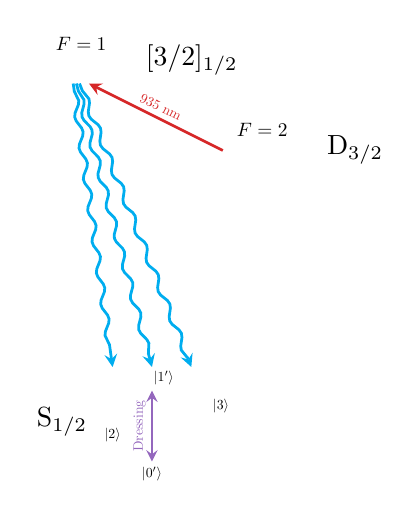
\begin{tikzpicture}
  % Zeeman
  \def\Zx{0.5}
  \def\Zy{0.1}

  % S
  \def\Sx{0}
  \def\Sy{0}
  \def\Sh{0.6}
  \def\Sdh{0.9}

  % D
  \def\Dx{0.9}
  \def\Dy{3.8}

  % Bracket
  \def\Bx{-0.9}
  \def\By{5}

  % Bracket
  \node[right] at (\Bx+\Zx+0.2, \By+\Zy) {$[3/2]_{1/2}$};
  \node[above] at (\Bx, \By+0.1) {\scalebox{0.7}{$F=1$}};
  \mytweezer.drawState(\Bx-\Zx, \By-\Zy)
  \mytweezer.drawState(\Bx, \By)
  \mytweezer.drawState(\Bx+\Zx, \By+\Zy)

  % D
  \node[right] at (\Dx+\Zx*2 + 0.2, \Dy+\Zy*2-0.05) {$\mathrm{D}_{3/2}$};
  \node[above] at (\Dx+\Zx, \Dy+0.2) {\scalebox{0.7}{$F=2$}};
  \mytweezer.drawState(\Dx-\Zx*2, \Dy-\Zy*2)
  \mytweezer.drawState(\Dx-\Zx, \Dy-\Zy)
  \mytweezer.drawState(\Dx, \Dy)
  \mytweezer.drawState(\Dx+\Zx, \Dy+\Zy)
  \mytweezer.drawState(\Dx+\Zx*2, \Dy+\Zy*2)

  \draw[pyplotc3, ->, >=stealth, line width=1]
  (\Dx, \Dy + 0.15) -- node[sloped,above=-0.05] {\scalebox{0.5}{$935\ \mathrm{nm}$}} (\Bx + 0.1, \By - 0.2);
  \draw[cyan, ->, snakearrow, >=stealth, line width=1]
  (\Bx - 0.1, \By - 0.2) -- (\Sx - \Zx, \Sy + 1.2);
  \draw[cyan, ->, snakearrow, >=stealth, line width=1]
  (\Bx - 0.06, \By - 0.2) -- (\Sx, \Sy + 1.2);
  \draw[cyan, ->, snakearrow, >=stealth, line width=1]
  (\Bx - 0.02, \By - 0.2) -- (\Sx + \Zx, \Sy + 1.2);

  % S
  \node[left] at (\Sx-\Zx-0.2, \Sy+\Sh-\Zy) {$\mathrm{S}_{1/2}$};
  \mytweezer.drawState(\Sx, \Sy+\Sdh)
  \mytweezer.drawState(\Sx-\Zx, \Sy+\Sh-\Zy)
  \mytweezer.drawState(\Sx+\Zx, \Sy+\Sh+\Zy)
  \mytweezer.drawState(\Sx, \Sy)
  \draw[pyplotc4, <->, >=stealth, line width=0.8]
  (\Sx, \Sy) -- node[sloped,above=-0.05] {\scalebox{0.5}{Dressing}} (\Sx, \Sy+\Sdh);

  \node[below=-0.05] at (\Sx, \Sy)
  {\scalebox{0.5}{$|0'\rangle$}};
  \node[above=-0.05] at (\Sx+0.15, \Sy+\Sdh)
  {\scalebox{0.5}{$|1'\rangle$}};
  \node[below=-0.05] at (\Sx-\Zx, \Sy+\Sh-\Zy)
  {\scalebox{0.5}{$|2\rangle$}};
  \node[right=-0.05] at (\Sx+\Zx+0.2, \Sy+\Sh+\Zy)
  {\scalebox{0.5}{$|3\rangle$}};

  \mytweezer.drawAtom(\Sx, \Sy+\Sdh, 0.17, pyplotc1)
  \mytweezer.drawAtom(\Sx-\Zx, \Sy+\Sh-\Zy, 0.09, pyplotc0)
  \mytweezer.drawAtom(\Sx+\Zx, \Sy+\Sh+\Zy, 0.09, pyplotc0)
  \mytweezer.drawAtom(\Sx, \Sy, 0.09, pyplotc0)
\end{tikzpicture}
\end{document}
